\documentclass[a4paper]{article}

\usepackage[english]{babel}
\usepackage[utf8]{inputenc}
\usepackage{amsmath}
\usepackage{graphicx}
\usepackage{listings}
\lstset{language=R} 
\usepackage[colorinlistoftodos]{todonotes}

\title{Persistent Homology Testing}
\author{Mike Wu}
\date{\today}

\begin{document}
\maketitle

The goal of this exercise is to test different types of topological analysis on a fake dataset created from sampling many uniform circles. Because a circle is made up of a single loop and void, it serves as a good baseline to differentiate the methods. 

\section{Setup}
Each of the following diagrams are generated via $N$ simulations of sampling $n$ times from an uniform circle of radius $r$ and center $(c_{0}, c_{1})$. Many of the functions used in the diagrams come from R's topological data analysis library. 

\begin{lstlisting}
circle <- function(num=n, rad=r, center=c(0, 0)) {
  x0 <- center[1] 
  y0 <- center[2]
  u <- 2 * pi * runif(num)
  result <- rad * cbind(x = cos(u) + x0, y = sin(u) + y0)
  return(result)
}
\end{lstlisting}

\section{RIPS Diagram}
\noindent For each of the $N$ simulations, it would be informative to plot the RIPS diagram for each N simulation overlayed on top of one another. By doing so should shed light on groups of 0-dimensional, and 1-dimensional objects like voids and loops. 

\begin{lstlisting}
multiRIPS <- function(maxdimension, maxscale, N, K) {
  for (i in 1:N) {
    Circle <- circle(K, radius, center)
    Diag <- ripsDiag(Circle, maxdimension, maxscale, 
    		     library = "GUDHI", printProgress = FALSE)
    par(new = TRUE)
    plot(Diag$diagram, main = "RIPS Diagram")
  }
}
\end{lstlisting}

\noindent An example of usage of multiRIPS:
\begin{lstlisting}
maxdimension <- 1        # components and loops
maxscale     <- 5        # limit of the filtration
radius       <- 2        # radius of circle
center       <- c(0, 0)  # center of circle
multiRIPS(maxdimension, maxscale, 10, 100)
\end{lstlisting}
For all RIPS plots, maxdimension is set to 1, and maxscale is set to 5. We are only looking for loops, and limit filtration to 5. Circles are centered at the origin, with a radius of 2, 100 samples are drawn, and 10 simulations are conducted. 

\begin{center}
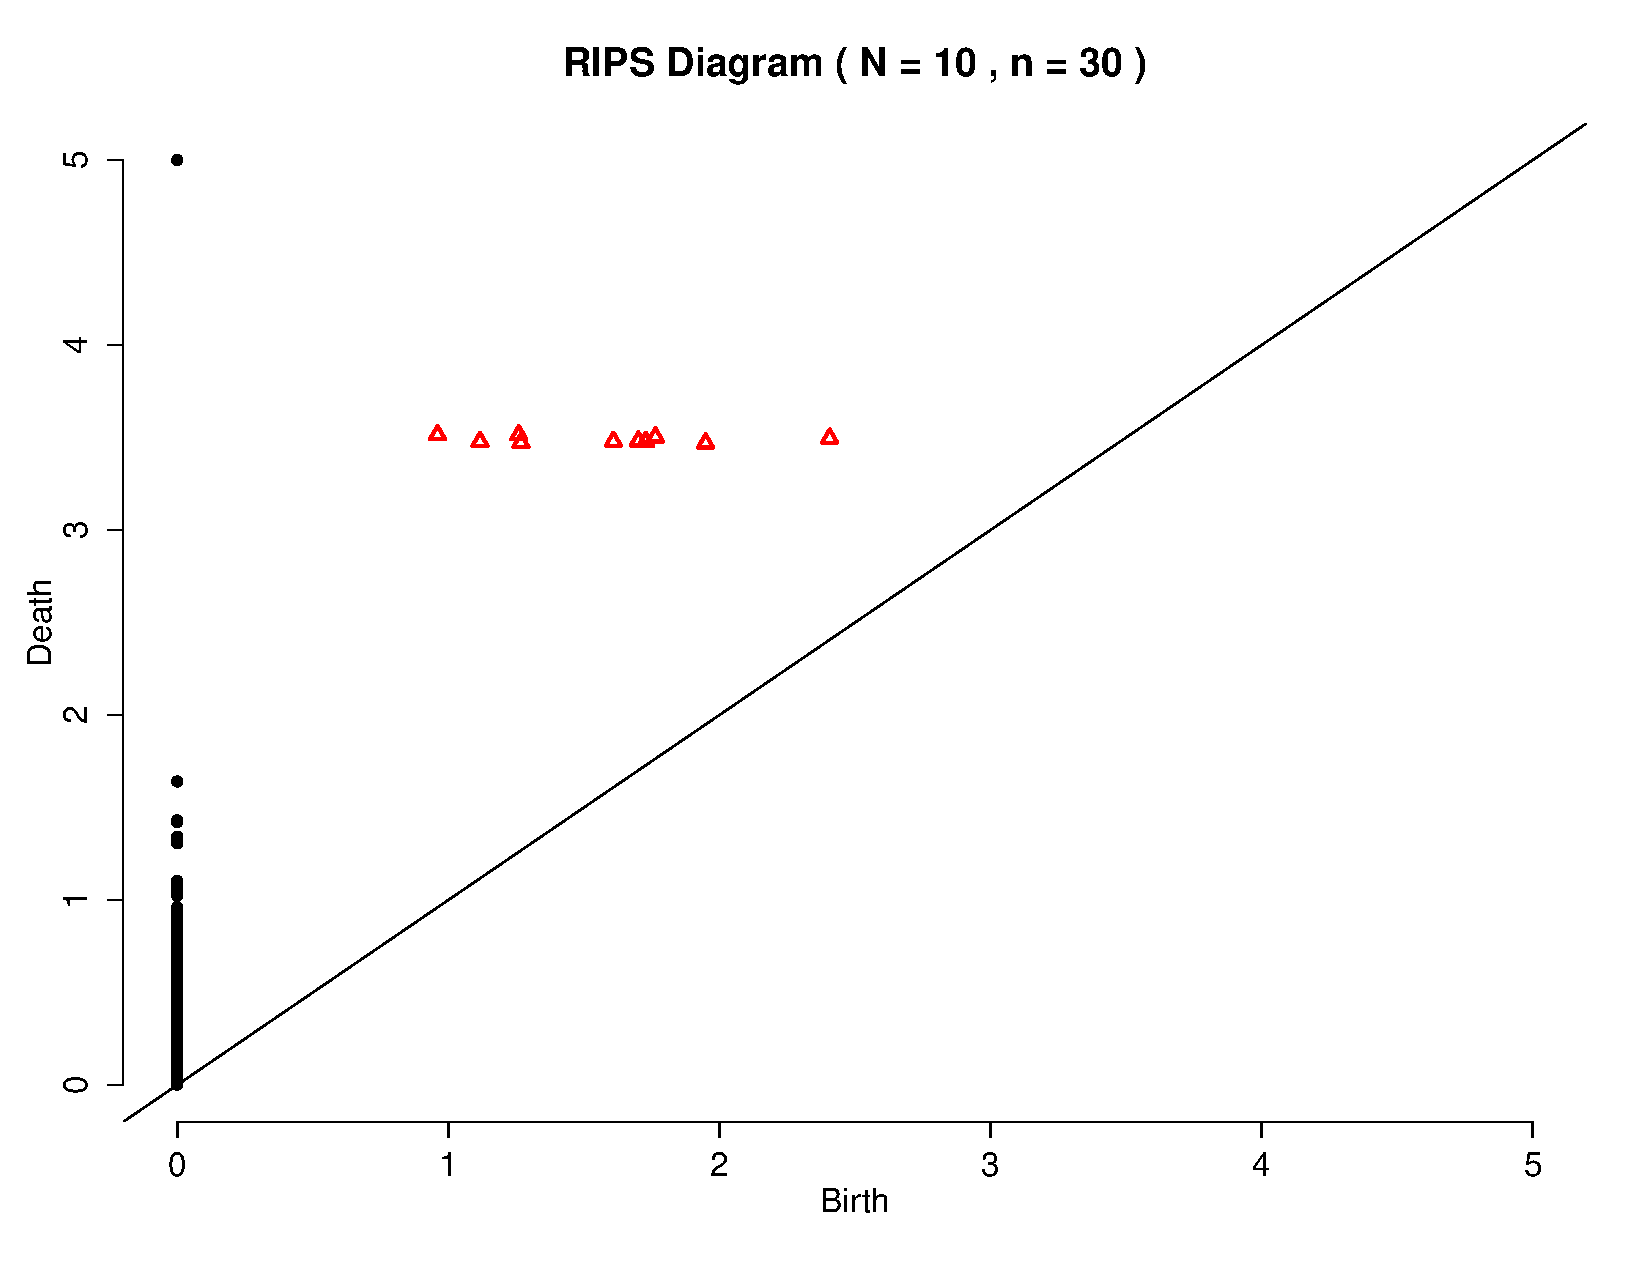
\includegraphics[width=0.55\linewidth]{RIPS_n30.pdf}
\end{center}

\noindent More interesting is to see what happens when $n$, the number of points sampled for each circle, varies (i.e. $n$ = 10, 100, 1000, ...). Intuitively, I would expect a smaller $n$ to less perfectly represent a circle, possibly making it more difficult to find the correct loops and voids. As $n$ grows large, the shape and characteristics of the circle should be more readily available. \newline

\begin{figure}[!htb]
\minipage{0.50\textwidth}
  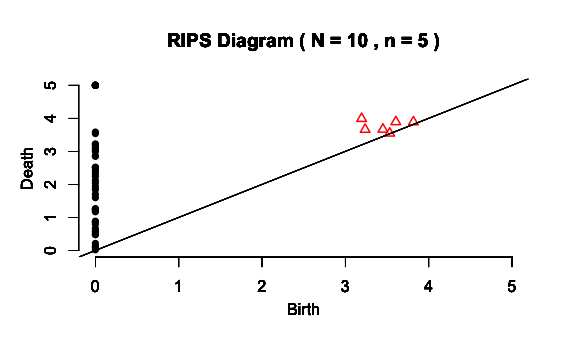
\includegraphics[width=\linewidth]{RIPS_5n.png}
\endminipage\hfill
\minipage{0.50\textwidth}
  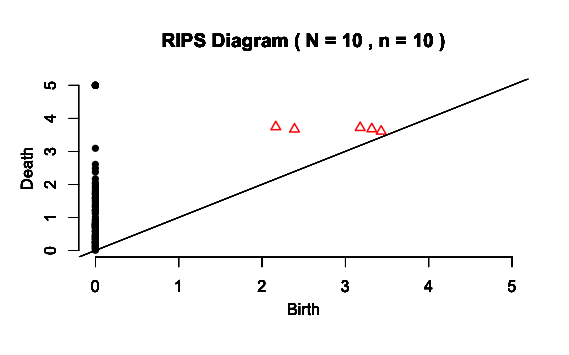
\includegraphics[width=\linewidth]{RIPS_10n.png}
\endminipage\hfill
\minipage{0.50\textwidth}
  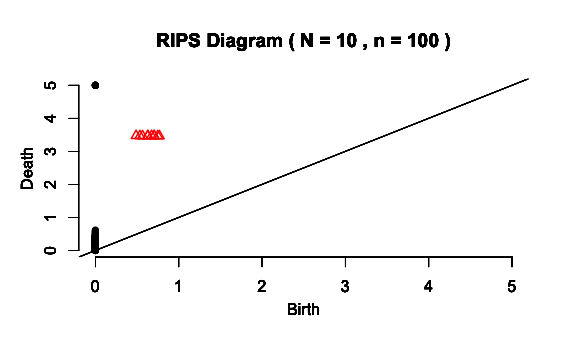
\includegraphics[width=\linewidth]{RIPS_n100.png}
\endminipage\hfill
\minipage{0.50\textwidth}
  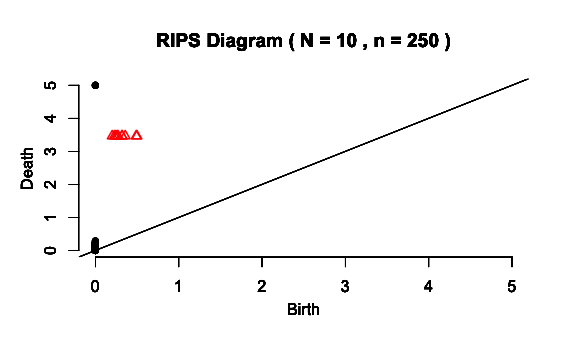
\includegraphics[width=\linewidth]{RIPS_n250.png}
\endminipage\hfill
\caption{Plots of overlapping RIPS diagrams. The number of simulations(N) is held constant but the sample size is varied (n).}
\end{figure}

\noindent Something interesting is that growing from n = 5, to n = 10 to n = 100, the program gets much slower. I think ripsDiag as a function does not scale linearly. This makes sense since with a large point cloud, growing individual balls at each point and running linear algebraic operations throughout is an expensive procedure. \newline

\noindent Two immediate recognizable patterns are that (1) the greater the sample size (bigger $n$), the earlier the detection (and formation) of higher dimensional simplicial complexes. For example, when $n = 250$, the loop is detected as early as 0.1 units after birth, while when $n = 5$, the loop is detection after 3.5 units..., and (2), as $n$ grows larger, the amount of spread of deaths as time 0 is more concentrated. Compare the black dots when $n = 5$ to when $n = 250$. Intuitively, these observations make a lot of sense. Because there are more points, the circle is better interpolated, meaning that more points lie on the circle's perimeter. When the balls begin to grow, the amount of growth needed to form all the overlaps to find the circle is small. Thus, the loop is found immediately. When there are very few points, the balls need much longer to grow to overlap! An interesting conclusions from this is that given any 3 random points, there will be a loop found, even if there isn't actual structure to those three points. But most likely, that structure would not persist over time. The second observation is also explainable by the sample size. With more points, fewer initial 0-dimensional complexes appear (points), because points start out close enough to form longer segments. When $n$ is small, the points are individual complexes, leading to increased deaths.

\begin{figure}[!htb]
\minipage{0.32\textwidth}
  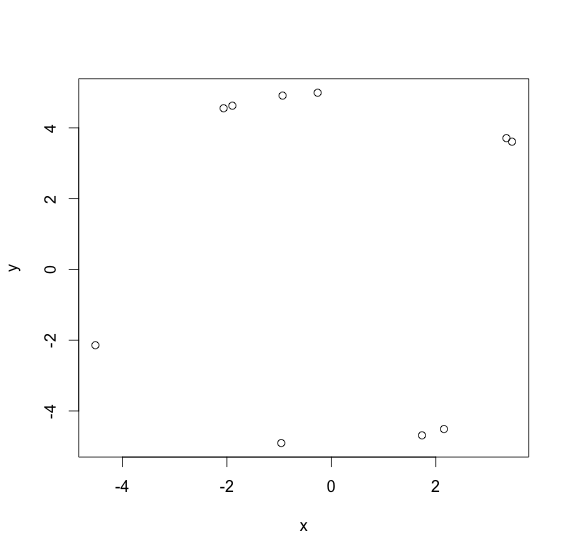
\includegraphics[width=\linewidth]{circle10.png}
\endminipage\hfill
\minipage{0.32\textwidth}
  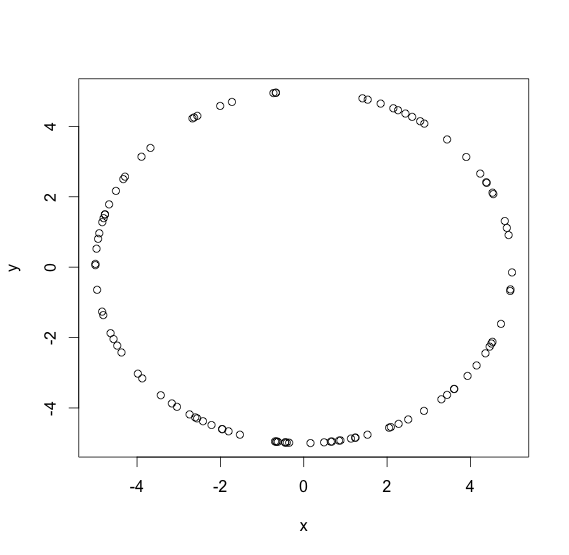
\includegraphics[width=\linewidth]{circle100.png}
\endminipage\hfill
\minipage{0.32\textwidth}
  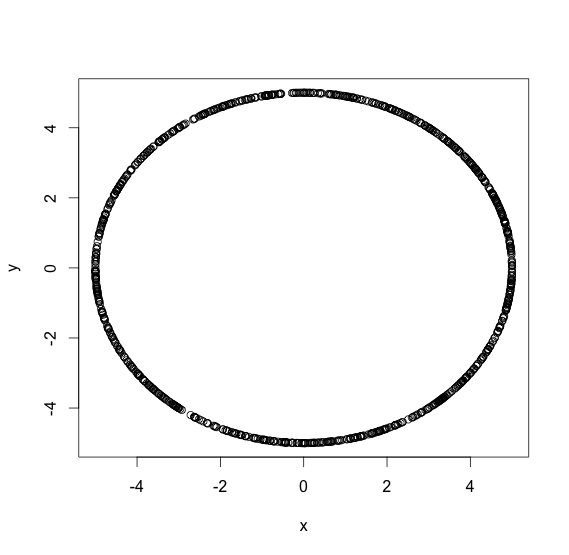
\includegraphics[width=\linewidth]{circle1000.png}
\endminipage\hfill
\caption{Plots of generated circles of different sample sizes.}
\end{figure}

\section{KDE Diagram}
A comparable series of operations can be done for Kernel Density Estimates in lieu of RIPS diagrams. 

\begin{lstlisting}
multiKDE <- function(N, Xlim, Ylim, by, h=0.3) {
  for (i in 1:N) {
    Circle <- circle(numparticle, radius, center)
    Diag <- gridDiag(X = Circle, FUN = kde, lim = cbind(Xlim, Ylim), 
                     by = by, sublevel = FALSE, library = "Dionysus"
                     printProgress = FALSE, h = h)
    par(new = TRUE)
    plot(Diag$diagram, main = "KDE Diagram")
  }
}
\end{lstlisting}

\noindent An example of usage of multiKDE:
\begin{lstlisting}
numparticle <- 10
radius      <- 2      
center      <- c(0, 0)
X           <- circle(numparticle, radius, center)
Xlim        <- c(center[1] - radius - 1, center[2] + radius + 1)
Ylim        <- c(center[1] - radius - 1, center[2] + radius + 1)
by          <- 0.1
multiKDE(10, Xlim, Ylim, by, 0.3)
\end{lstlisting}

\noindent The same plots ($n$ = 5, 10, 100, 1000) are generated for KDE: Again, circles are centered at the origin, with a radius of 2, and 10 simulations are conducted. Distance algorithms require a grid size. Our grid is defined by a box with a side length of radius + 1. The step size for the grid is set to 0.1. 0.3 is passed as the smoothing parameter for the gaussian kernel.  \newline

\begin{figure}[!htb]
\minipage{0.50\textwidth}
  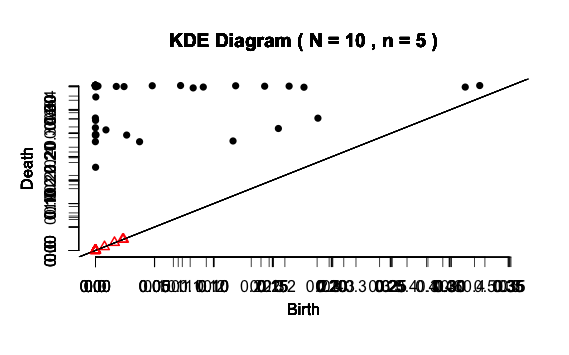
\includegraphics[width=\linewidth]{KDE_n5.png}
\endminipage\hfill
\minipage{0.50\textwidth}
  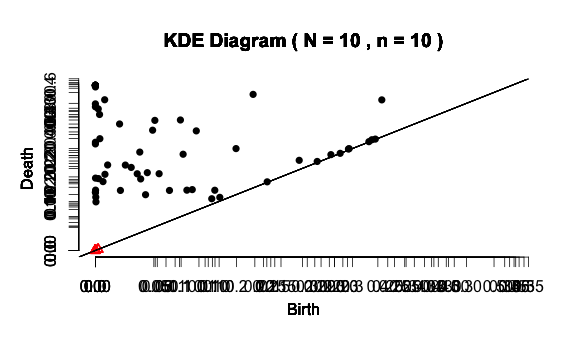
\includegraphics[width=\linewidth]{KDE_n10.png}
\endminipage\hfill
\minipage{0.50\textwidth}
  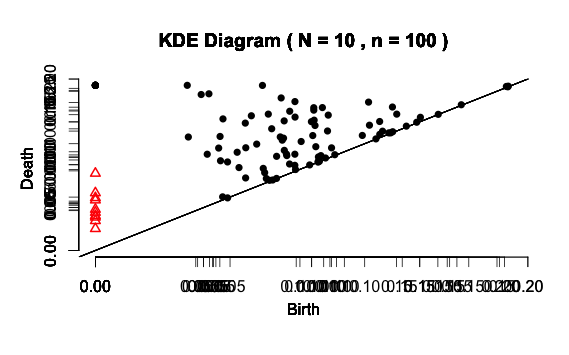
\includegraphics[width=\linewidth]{KDE_n100.png}
\endminipage\hfill
\minipage{0.50\textwidth}
  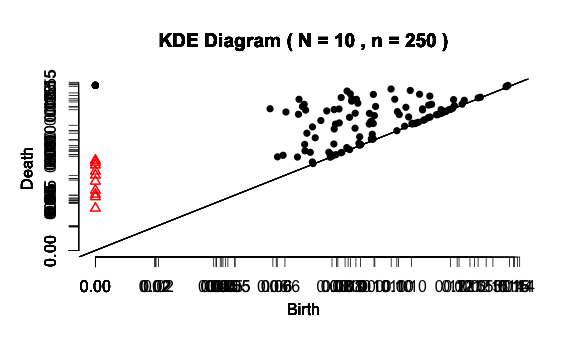
\includegraphics[width=\linewidth]{KDE_n250.png}
\endminipage\hfill
\caption{Plots of overlapping KDE diagrams. The number of simulations(N) is held constant but the sample size is varied (n).}
\end{figure}

\noindent Computationally, this method is less expensive than RIPS. The same setup of 10 simulations of 250 samples each was noticeably faster. 

\section{DTM Diagram}
Another possible algorithm to try is Distance to Measure. Let's repeat the process for this and see what happens. The settings are identical to the settings for KDE. Additionally, $m_{0}$ (the smoothing parameter for DTM aka for each point in the grid, when calculating distance, $m_{0}*100$\% of all points are considered) is set to 0.1. 

\begin{lstlisting}
multiDTM <- function(N, Xlim, Ylim, by, m0=0.1) {
  for (i in 1:N) {
    Circle <- circle(numparticle, radius, center)
    Diag <- gridDiag(X = Circle, FUN = dtm, lim = cbind(Xlim, Ylim), 
                     by = by, sublevel = FALSE, library = "Dionysus", 
                     printProgress = FALSE, m0 = m0)
    par(new = TRUE)
    plot(Diag$diagram, main = "DTM Diagram")
  }
}
\end{lstlisting}

\noindent Usage of multiDTM is very comparable to multiKDE. 

\section{Adding Noise}
Real datasets are not this perfect. They are often muddled with noise and overlapping objects. In this small extension, let's pick a reasonably defined circle (n = 250), use RIPS, and perturb the matrix with differing levels of noise. To what extent will proper objects still be found? Persistent Homology seems to give all points in the point cloud equal weight. If that is true, will small amounts of noise prevent us from finding the real object? 
\end{document}